\documentclass{article}

% [final] = camera-ready layout: shows author names, no line numbers
\usepackage[final]{neurips_2025}

\usepackage[utf8]{inputenc}
\usepackage[T1]{fontenc}
\usepackage{hyperref}
\usepackage{url}
\usepackage{booktabs}
\usepackage{amsfonts}
\usepackage{amsmath}
\usepackage{nicefrac}
\usepackage{microtype}
\usepackage{xcolor}
\usepackage{graphicx}
\usepackage{subcaption}
\usepackage{tikz}
\usetikzlibrary{positioning, arrows.meta, calc}
\definecolor{ours}{HTML}{2A78D6}

% Course report, not a NeurIPS paper: replace the "39th Conference on NeurIPS"
% footer that the [final] option prints, and drop hyperref's coloured boxes.
\makeatletter
\renewcommand{\@noticestring}{Course project report, Computer Vision, IIT Jodhpur, November 2026.}
\makeatother
\hypersetup{colorlinks=true, linkcolor=black, citecolor=blue!50!black, urlcolor=blue!50!black}

% marks numbers that are still being computed; must be empty before submission
\newcommand{\pending}[1]{\textcolor{red}{\textbf{[#1]}}}

\title{Hough-SIFT: Hough Pose Clustering for\\Learned Local Features with Semantic-Gated Voting}

\author{%
  Rahul Kumar Bhikundia \\
  M26CSA006 \\
  IIT Jodhpur \\
  \texttt{m26csa006@iitj.ac.in} \\
  \And
  Suggu Chandu \\
  M26CSA017 \\
  IIT Jodhpur \\
  \texttt{m26csa017@iitj.ac.in} \\
  \And
  Navneet Singh \\
  M26CSA004 \\
  IIT Jodhpur \\
  \texttt{m26csa004@iitj.ac.in} \\
}

\begin{document}

\maketitle

% =====================================================================
\begin{abstract}
Geometric verification of local feature matches is almost always done with
RANSAC, whose success probability collapses as the outlier ratio grows. Lowe's
Hough pose clustering is a deterministic alternative that is robust to
outliers, but it requires every keypoint to carry a scale and an orientation,
which learned detectors such as DISK and SuperPoint do not provide. We make
Hough verification usable with orientation-free features through
\emph{pairwise similarity voting}: two correspondences determine a full
similarity transform, so neighbouring pairs of matches cast the votes. Naive
pairwise voting collapses under heavy contamination; we diagnose why (wrong
matches produce absurd-scale votes that pile up in oversized location bins)
and fix it with a scale prior and a mutual-spatial-neighbour rule. On HPatches
(580 pairs) our verifier is on par with MAGSAC++ up to 90\% injected outliers
and clearly ahead at 95\% (75.2\% vs.\ 36.9\% of pairs within 3\,px with
SIFT, 51.4\% vs.\ 33.8\% with DISK). We then study \emph{semantic-gated Hough
voting}, in which Mask R-CNN instance masks decide which matches may vote
together and the instance identity becomes an extra Hough dimension. On a
synthetic multi-object benchmark built from COCO, with design choices made on
a held-out validation split, gating plus duplicate merging keeps object
recall almost constant from 0\% to 80\% outliers (74.3\% to 72.7\% with DISK)
while sequential RANSAC drops from 85.4\% to 19.0\%, and at 80\% outliers it
produces 4$\times$ fewer wrong hypotheses than semantic RANSAC at 17$\times$
lower cost. On clean scenes, plain RANSAC remains the best choice; we report
this and the variants that did not work.
\end{abstract}

% =====================================================================
\section{Introduction}

Matching local features between two images is a basic step in object
recognition, image stitching, visual localisation and structure from motion.
Descriptor matching always returns a mixture of correct and incorrect
correspondences, so a \emph{geometric verification} step must decide which
matches are consistent with a single physical motion. The standard tool is
RANSAC~\cite{fischler1981ransac} and its modern variants such as
MAGSAC++~\cite{barath2020magsacpp}: repeatedly sample a minimal set of matches,
fit a model and count agreeing matches. RANSAC's weakness is well known. A
minimal sample of four matches is outlier-free with probability
$(1-\varepsilon)^4$ for outlier ratio $\varepsilon$, which is $10^{-4}$ at
$\varepsilon=0.9$, so the number of required iterations explodes exactly in
the hard cases.

Lowe's object recognition system~\cite{lowe2004sift} used a different
strategy: every SIFT match votes for an object pose (scale, rotation and
position) in a coarse Hough accumulator~\cite{duda1972hough,ballard1981ght}.
Correct matches agree and form a peak; incorrect matches spread their votes
thinly across pose space. Voting is deterministic, uses each match once and
degrades gracefully with outliers. Hough verification has, however, largely
disappeared from modern pipelines built on learned features. Benchmarks of
learned matchers still verify with RANSAC~\cite{yu2024gvbench}. One reason is
structural: a single SIFT match can vote because each SIFT keypoint carries
its own scale and orientation. Learned detectors such as
DISK~\cite{tyszkiewicz2020disk} and SuperPoint~\cite{detone2018superpoint}
output only a 2-D location, so a single match no longer determines a pose.

A second weakness of classical Hough voting appears in cluttered scenes:
\emph{any} two matches may vote together, so a pair spanning two different
objects casts a meaningless vote, and two objects with similar motion can
merge into one cluster. Semantic segmentation knows which pixels belong to
which object, which is exactly the information needed to prevent this.

\paragraph{Contributions.}
\begin{enumerate}
  \item \textbf{Pairwise similarity voting for orientation-free features.} We
  adapt Lowe-style Hough verification to learned detectors by letting pairs of
  neighbouring matches vote, since two correspondences determine scale and
  rotation. We identify why naive pairwise voting collapses under heavy
  contamination and fix it with a scale prior and a mutual-spatial-neighbour
  rule.
  \item \textbf{Semantic-gated Hough voting.} Instance masks from an
  off-the-shelf segmenter decide which matches may vote together, and the
  instance identity becomes an additional Hough dimension, so votes from
  different objects never share a bin. A \emph{soft} rule treats background
  as ``unknown'', and duplicate merging removes the redundant hypotheses that
  gating creates. We show that gating and voting are complementary: under heavy
  clutter the combination outperforms either component alone.
  \item \textbf{Evaluation, including negative results.} An outlier-injection
  study on HPatches~\cite{balntas2017hpatches} against RANSAC and
  MAGSAC++~\cite{barath2020magsacpp}, a sensitivity analysis of the
  neighbourhood size, and a $2\times2\times2$ ablation on a synthetic
  multi-object benchmark built from COCO~\cite{lin2014coco} with ground-truth
  motion for every object, with a separate validation split for design
  decisions. We also report the variants that failed and why.
\end{enumerate}

% =====================================================================
\section{Literature Review}

\paragraph{Hough-based geometric verification.}
The Hough transform~\cite{duda1972hough} and its generalisation to arbitrary
shapes~\cite{ballard1981ght} turn model fitting into peak finding in a
parameter space. Lowe~\cite{lowe2004sift} applied it to SIFT matches with a
4-D similarity pose space and coarse bins (30$^\circ$ orientation, factor 2 in
scale, a quarter of the model size in location), followed by least-squares
affine refinement. Hough pyramid matching~\cite{tolias2011hpm} relaxes the
quantisation with a hierarchy of bin sizes, and the vote-and-verify strategy
of Sch\"onberger et al.~\cite{schonberger2016vote} combines voting with
hypothesis verification for fast spatial verification in retrieval. All of
these rely on per-keypoint scale and orientation.

\paragraph{Robust estimation by sampling.}
RANSAC~\cite{fischler1981ransac} remains the default verifier. MAGSAC++
\cite{barath2020magsacpp} removes the need for a hand-tuned inlier threshold
by marginalising over noise scales and is among the strongest classical
estimators. Multi-model problems (several independently moving objects) are
commonly handled by sequential RANSAC or energy-based methods such as
PEARL~\cite{isack2012pearl}.

\paragraph{Pairwise geometric consistency.}
Pairs of correspondences carry more geometry than single ones. Spectral
matching~\cite{leordeanu2005spectral} scores pairwise consistency between
matches, Li et al.~\cite{li2015pairwise} use pairwise geometric relations for
large-scale object retrieval, and GMS~\cite{bian2017gms} rejects matches whose
spatial neighbourhoods are not preserved between images. Our pairwise voting
and our mutual-neighbour rule build on the same intuition, applied inside a
Hough accumulator for learned features.

\paragraph{Learned local features.}
SuperPoint~\cite{detone2018superpoint}, D2-Net~\cite{dusmanu2019d2net} and
DISK~\cite{tyszkiewicz2020disk} learn detection and description jointly and
outperform SIFT on many benchmarks; learned matchers such as
LightGlue~\cite{lindenberger2023lightglue} further improve the matching step.
These detectors provide keypoint locations without scale or orientation, and
their downstream verification is almost always RANSAC~\cite{yu2024gvbench}.

\paragraph{Segmentation-guided matching.}
The closest prior work is the co-segmentation guided Hough transform of Chen
et al.~\cite{chen2015coseghough}, which uses unsupervised co-segmentation of
an image pair to select relevant voters in a Hough space of homographies.
SGAM~\cite{zhang2023sgam} first matches semantic areas and then points inside
matched areas; MESA~\cite{zhang2024mesa} replaces semantic labels with Segment
Anything~\cite{kirillov2023sam} masks and reports that SGAM degrades with
inexact semantic labels. Our work differs from these in three ways: we use
\emph{instance} segmentation from a pretrained detector (Mask
R-CNN~\cite{he2017maskrcnn}) to handle several objects, we encode instance
identity as an additional Hough dimension rather than only filtering voters,
and we explicitly design for segmentation failures with a soft gating rule,
which we evaluate against a strict variant.

% =====================================================================
\section{Problem Statement}

Given two images $I_1, I_2$ and a set of putative correspondences
$\mathcal{M} = \{(\mathbf{p}_i, \mathbf{q}_i)\}_{i=1}^{M}$, where
$\mathbf{p}_i \in I_1$ and $\mathbf{q}_i \in I_2$ are keypoint locations
produced by a detector and descriptor matching, a fraction $\varepsilon$ of
which are incorrect, we address two tasks.

\paragraph{Task 1: single-model verification.} Estimate the homography
$\mathbf{H}$ relating a planar scene in $I_1$ and $I_2$ and the set of inlier
correspondences, when keypoints carry no scale or orientation. Accuracy is
measured by the mean corner error
$e = \tfrac14 \sum_{c=1}^{4} \lVert \pi(\mathbf{H}\mathbf{c}_c) -
\pi(\mathbf{H}^{\ast}\mathbf{c}_c)\rVert$ between the image corners
$\mathbf{c}_c$ mapped by the estimate and by the ground truth
$\mathbf{H}^{\ast}$, where $\pi$ denotes dehomogenisation. We report the
percentage of image pairs with $e < 1, 3, 5$ pixels, and study how it changes
as $\varepsilon$ grows.

\paragraph{Task 2: multi-object verification.} The scene contains a background
and $K$ objects, each moving with its own homography
$\mathbf{H}^{\ast}_0, \ldots, \mathbf{H}^{\ast}_K$. Recover one hypothesis per
motion without producing hypotheses that mix matches from different objects.
We measure object recall, the number of false hypotheses per image, and
cluster purity (Section~\ref{sec:multiobj}).

% =====================================================================
\section{Proposed Method}

Figure~\ref{fig:pipeline} summarises the pipeline: feature extraction and
matching, Hough voting, cluster verification, and optional semantic gating.

\begin{figure}[t]
  \centering
  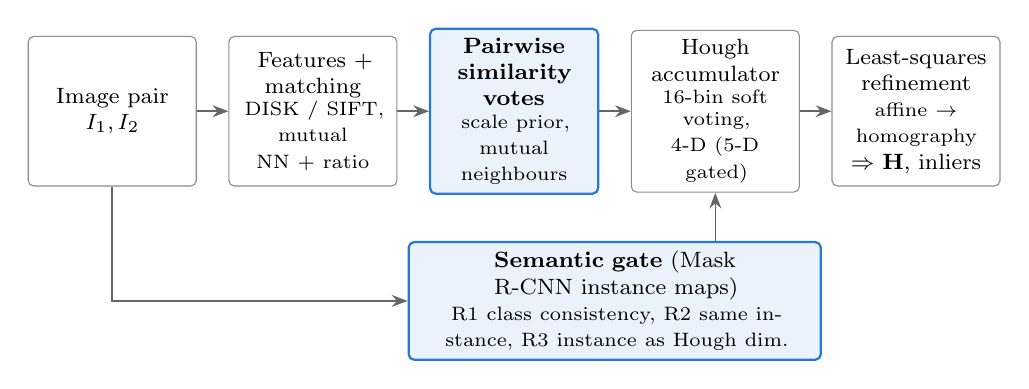
\begin{tikzpicture}[
      font=\footnotesize, node distance=4mm,
      box/.style={draw=black!45, rounded corners=2pt, align=center,
                  text width=19mm, minimum height=19mm, fill=white},
      ours/.style={box, draw=ours, fill=ours!10, line width=0.8pt},
      arr/.style={-{Stealth[length=2mm]}, black!60, line width=0.6pt}]
    \node[box]  (img)  {Image pair\\$I_1, I_2$};
    \node[box,  right=of img]  (feat) {Features +\\matching\\{\scriptsize DISK / SIFT,\\mutual NN + ratio}};
    \node[ours, right=of feat] (vote) {\textbf{Pairwise}\\\textbf{similarity votes}\\{\scriptsize scale prior,\\mutual neighbours}};
    \node[box,  right=of vote] (hough){Hough\\accumulator\\{\scriptsize 16-bin soft voting,\\4-D (5-D gated)}};
    \node[box,  right=of hough](ref)  {Least-squares\\refinement\\{\scriptsize affine $\to$ homography}\\$\Rightarrow \mathbf{H}$, inliers};
    \node[ours, anchor=north, text width=50mm, minimum height=9mm] (gate)
         at ($(vote.south)!0.5!(hough.south) + (0,-6mm)$)
         {\textbf{Semantic gate} (Mask R-CNN instance maps)\\{\scriptsize R1 class consistency, R2 same instance, R3 instance as Hough dim.}};
    \draw[arr] (img) -- (feat);
    \draw[arr] (feat) -- (vote);
    \draw[arr] (vote) -- (hough);
    \draw[arr] (hough) -- (ref);
    \draw[arr] (img.south) |- (gate.west);
    \draw[arr] (gate.north -| hough.south) ++(0,0) -- (hough.south);
  \end{tikzpicture}
  \caption{Overview of the proposed verification pipeline. Blue boxes are our contributions; the semantic gate is optional and only used for multi-object scenes.}
  \label{fig:pipeline}
\end{figure}

\subsection{Features and matching}
We use DISK~\cite{tyszkiewicz2020disk} (pretrained ``depth'' weights via
Kornia~\cite{riba2020kornia}) as the learned detector and SIFT with RootSIFT
normalisation~\cite{arandjelovic2012rootsift} as the classical baseline, with
up to 4000 keypoints per image. Matches are mutual nearest neighbours that
also pass Lowe's ratio test (0.8 for SIFT, 0.95 for DISK, whose descriptor
distances are less peaked).

\subsection{Hough voting for a similarity pose}
A similarity transform has four parameters: scale $s$, rotation $\theta$ and a
2-D translation. Following Lowe~\cite{lowe2004sift}, translation is not voted
as raw $(t_x, t_y)$, which depends on the choice of origin, but as the
predicted position of the centre $\mathbf{c}_1$ of $I_1$ in $I_2$:
\begin{equation}
  \mathbf{c}_2 = \mathbf{q}_a + s\,\mathbf{R}(\theta)\,(\mathbf{c}_1 - \mathbf{p}_a),
  \label{eq:centre}
\end{equation}
where $(\mathbf{p}_a, \mathbf{q}_a)$ is an anchor correspondence. Every
correct match on a rigid planar object predicts the same $\mathbf{c}_2$. Bins
are 30$^\circ$ in $\theta$, a factor of 2 in $s$, and
$0.25\cdot\max(h_1,w_1)\cdot s$ in location. Each vote is cast into the two
nearest bins along every dimension ($2^4 = 16$ bins) so that a pose near a
bin boundary is not split. A cluster's support is the number of
\emph{distinct} matches that voted for it.

\paragraph{Single-match votes (SIFT).} With keypoint scales $\sigma$ and
orientations $\phi$, a single match gives $s = \sigma'/\sigma$ and
$\theta = \phi' - \phi$, and serves as its own anchor.

\paragraph{Pairwise votes (learned features).} DISK keypoints have no $\sigma$
or $\phi$. Two matches $i, j$, however, define the segments
$\mathbf{u} = \mathbf{p}_j - \mathbf{p}_i$ and
$\mathbf{v} = \mathbf{q}_j - \mathbf{q}_i$, and
\begin{equation}
  s = \frac{\lVert\mathbf{v}\rVert}{\lVert\mathbf{u}\rVert},\qquad
  \theta = \operatorname{atan2}(\mathbf{v}) - \operatorname{atan2}(\mathbf{u}),
  \label{eq:pair}
\end{equation}
which, together with Eq.~\eqref{eq:centre} using match $i$ as anchor, is a
complete similarity vote supporting both $i$ and $j$. Each match is paired
with its $k$ nearest matched neighbours in $I_1$, since nearby points are
likely to lie on the same surface; pairs closer than 10\,px are skipped
because short segments give unstable angles.

\paragraph{Making pairwise voting robust.} Naive pairwise voting fails under
heavy contamination (Section~\ref{sec:outliers}). The cause is specific to
pairs. A wrong match $j$ that lies near $i$ in $I_1$ lands at an arbitrary
position in $I_2$, so $\lVert\mathbf{v}\rVert \gg \lVert\mathbf{u}\rVert$ and
Eq.~\eqref{eq:pair} implies an absurd scale. Because location bins grow with
scale, such votes fall into a few very large bins and form fake peaks: at
80\% outliers, 88\% of all pair votes implied scales outside $[1/8, 8]$ and
the winning cluster had a median scale of 15--34 while the true scale was
close to 1. We add two rules:
\begin{itemize}
  \item \textbf{Scale prior:} votes with $s \notin [1/8, 8]$ are discarded.
  \item \textbf{Mutual spatial neighbours:} a pair is kept only if $j$ is also
  among the $2k$ nearest neighbours of $i$ in $I_2$. A rigid object preserves
  neighbourhoods; a random wrong match almost never does (cf.\ GMS~\cite{bian2017gms}).
\end{itemize}

\subsection{Cluster verification}
A Hough bin is coarse, so each of the top 10 clusters is refined by iterative
least squares with no random sampling: fit an affine transform to the
cluster, re-collect \emph{all} matches with reprojection error below 10\,px,
switch to a full homography (direct linear transform, least squares) once at
least 8 inliers exist and tighten the threshold to 3\,px, and repeat until the
inlier set is stable. The cluster with the most final inliers is returned. The
procedure is deterministic: the same input always gives the same output.

\subsection{Semantic-gated voting}
We run a COCO-pretrained Mask R-CNN~\cite{he2017maskrcnn} (score $>0.5$) on
both images to obtain instance maps $\iota_1, \iota_2$ (0 = background) with
class labels $c(\cdot)$. Each match $m$ receives instance ids
$\iota_1(\mathbf{p}_m), \iota_2(\mathbf{q}_m)$. Three rules restrict voting:
\begin{itemize}
  \item \textbf{R1 (class consistency):} discard a match whose endpoints lie on
  objects of different classes.
  \item \textbf{R2 (same instance):} a pair may vote only if both matches lie on
  the same instance in $I_1$ and in $I_2$.
  \item \textbf{R3 (instance dimension):} the instance id is appended as a fifth
  Hough coordinate, so votes from different objects never share a bin, and
  verification of a cluster only collects inliers from its own instance.
\end{itemize}
\paragraph{Strict vs.\ soft gating.} In \emph{strict} mode background is an
ordinary label, so a match from a detected cup to an undetected region is
rejected by R1. In practice detections are often missed in one of the two
images, and strict gating then deletes real objects. In \emph{soft} mode,
background means ``unknown'': R1 rejects only when both endpoints are detected
\emph{and} disagree, R2 treats an unknown endpoint as compatible, and the
group used by R3 is the instance in $I_1$.

\subsection{Multi-object extraction and duplicate merging}
For multi-object scenes, hypotheses are extracted greedily: clusters are
visited in order of support (up to 300 clusters), each is refined as above
using only matches not yet claimed (and, with gating, only matches of the
cluster's instance group), and a hypothesis with at least 8 inliers claims
its matches. Gating splits a single motion into several groups when the
segmenter detects several ``stuff'' instances on the background (a table, a
wall), producing duplicate hypotheses for the same motion. We therefore
\emph{merge} a hypothesis into an earlier one whenever the earlier homography
already explains its inliers (median transfer error below 5\,px) and refit on
the union. Merging is applied identically to every method in our experiments.

% =====================================================================
\section{Experiments and Results}

\paragraph{Implementation.} Python with OpenCV, PyTorch and Kornia, on a
single NVIDIA GTX 1650 (4\,GB) under WSL2 with 4.8\,GB RAM. All Hough
parameters are fixed across experiments: Lowe's bin sizes, $k=16$, scale
prior $[1/8, 8]$, 3\,px final inlier threshold. Baselines are OpenCV's RANSAC
and USAC-MAGSAC (MAGSAC++), both with a 3\,px threshold, 10{,}000 iterations
and 0.999 confidence.

\subsection{Single-model verification on HPatches}
\label{sec:outliers}
HPatches~\cite{balntas2017hpatches} contains 116 planar scenes (57 with
illumination changes, 59 with viewpoint changes) of 6 images each, giving 580
pairs with ground-truth homographies. Images are resized to at most 1024\,px.
To test robustness we inject synthetic outliers: random correspondences with
uniformly random positions (and, for SIFT, random scales and orientations)
appended until a fraction $\varepsilon$ of all matches are wrong.

\begin{table}[t]
  \caption{HPatches, no injected outliers (580 pairs). Percentage of pairs with
  mean corner error below 1/3/5\,px, split by illumination (Illum) and
  viewpoint (View) scenes at 3\,px, and median verification time.}
  \label{tab:clean}
  \centering\small
  \begin{tabular}{llcccccr}
    \toprule
    Features & Verifier & @1px & @3px & @5px & Illum@3 & View@3 & ms \\
    \midrule
    SIFT & RANSAC              & 47.9 & 77.2 & 86.6 & 89.5 & 65.4 & 0.6 \\
    SIFT & MAGSAC++            & 52.6 & 81.4 & \textbf{89.0} & 90.2 & \textbf{72.9} & 0.4 \\
    SIFT & Hough, single~\cite{lowe2004sift} & \textbf{53.1} & \textbf{81.6} & 88.1 & \textbf{90.5} & \textbf{72.9} & 15.5 \\
    SIFT & Hough, pairwise (ours) & 52.6 & 80.7 & 87.2 & 89.8 & 71.9 & 34.3 \\
    \midrule
    DISK & RANSAC              & 42.8 & 74.7 & 85.0 & 91.9 & 58.0 & 0.9 \\
    DISK & MAGSAC++            & 53.8 & 82.6 & \textbf{90.0} & 96.5 & \textbf{69.2} & 1.1 \\
    DISK & Hough, pairwise (ours) & \textbf{55.2} & \textbf{82.9} & 88.6 & \textbf{97.2} & \textbf{69.2} & 128.9 \\
    \bottomrule
  \end{tabular}
\end{table}

\begin{figure}[t]
  \centering
  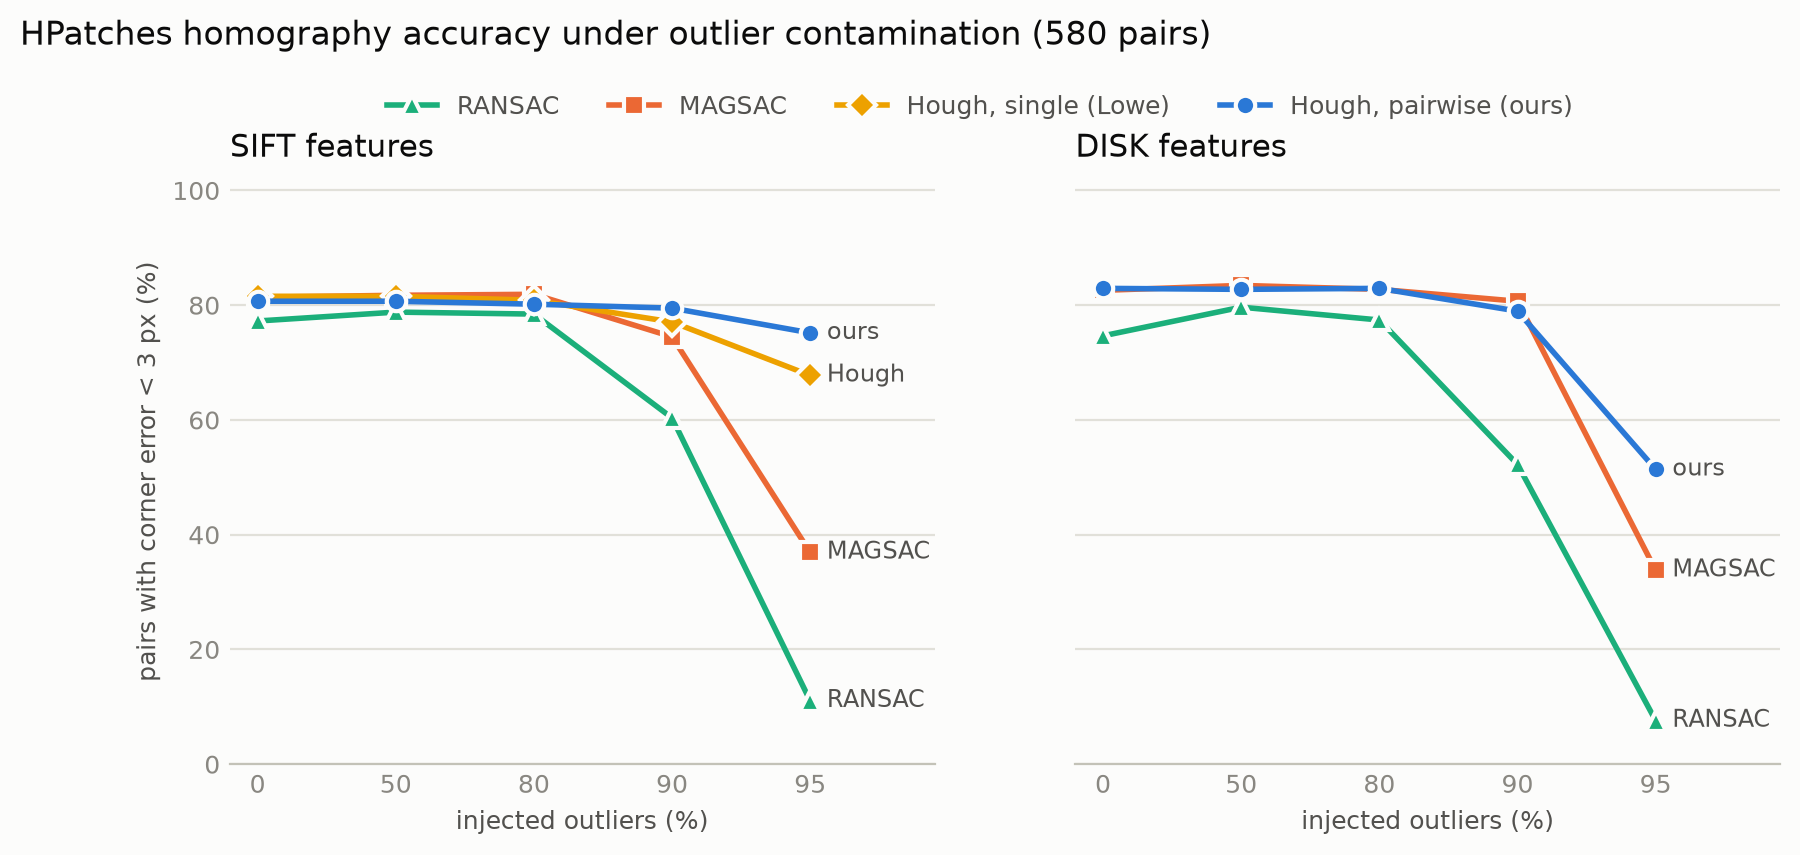
\includegraphics[width=\linewidth]{figures/fig_outliers.png}
  \caption{HPatches accuracy (pairs with corner error $<3$\,px) as synthetic
  outliers are injected. RANSAC collapses above 80\%; MAGSAC++ above 90\%.
  Pairwise Hough degrades gracefully.}
  \label{fig:outliers}
\end{figure}

\paragraph{Results without injected outliers.} Table~\ref{tab:clean} shows
that Hough verification is fully competitive on clean data. With DISK, our
pairwise verifier is the most accurate at 1\,px and 3\,px and on illumination
changes, and ties MAGSAC++ on viewpoint changes, while plain RANSAC trails by
8--13 points. With SIFT, pairwise voting (52.6/80.7) is within one point of
Lowe's single-match voting (53.1/81.6), which shows that discarding keypoint
scale and orientation costs essentially nothing once pairs are used. Our
pure-Python implementation is, however, 40--120$\times$ slower than OpenCV's
optimised C++ estimators on clean data.

\paragraph{Robustness to outliers.} Figure~\ref{fig:outliers} shows the main
result. Up to 80\% outliers all verifiers stay within a few points of their clean
accuracy. At 90\%,
RANSAC drops to 52--60\% while MAGSAC++ and pairwise Hough remain at 74--81\%.
At 95\%, MAGSAC++ falls to 36.9\% (SIFT) and 33.8\% (DISK), whereas pairwise
Hough retains 75.2\% and 51.4\%. With SIFT, pairwise voting even overtakes
Lowe's single-match voting at 95\% (75.2\% vs.\ 67.8\%): the
mutual-neighbour rule removes votes from random matches that single-match
voting has no way to reject.

\paragraph{Why naive pairwise voting failed.} Before adding the scale prior
and the mutual-neighbour rule, DISK with pairwise Hough fell from 83.3\% at
50\% outliers to 13.8\% at 80\%. Inspecting the accumulator showed that 88\%
of pair votes implied scales outside $[1/8, 8]$ and that the winning cluster
had a median implied scale of 15--34, against a true scale near 1. The two
rules raised accuracy at 80\% outliers back to 82.9\%.

\begin{figure}[t]
  \centering
  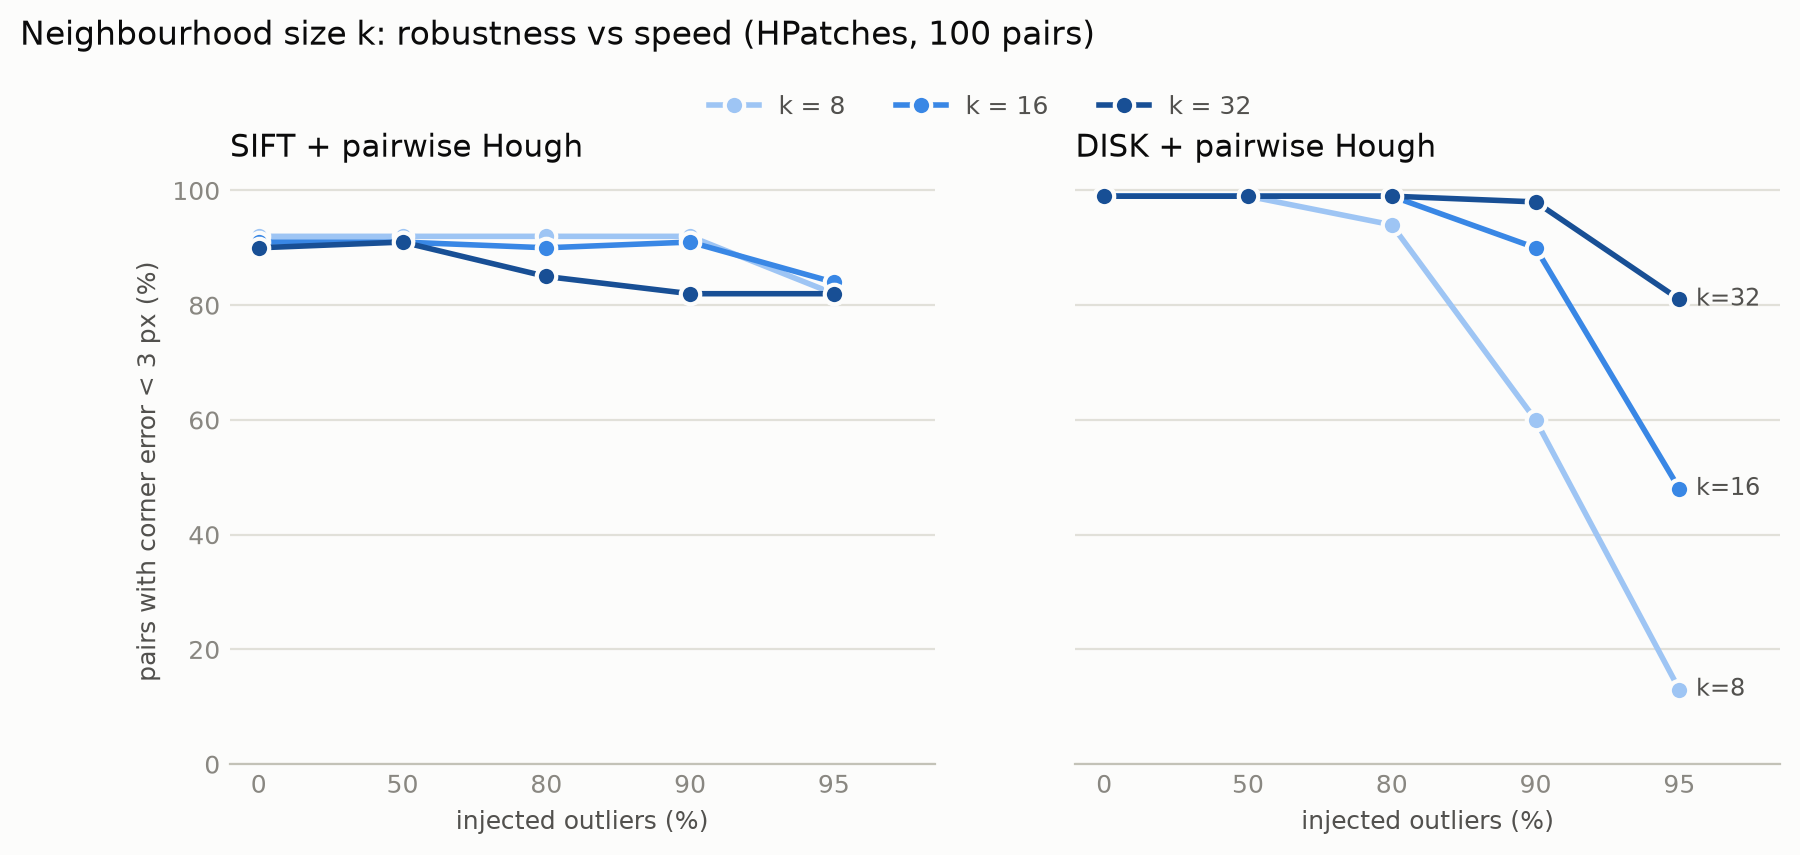
\includegraphics[width=\linewidth]{figures/fig_ksweep.png}
  \caption{Sensitivity of pairwise Hough to the neighbourhood size $k$
  (first 20 HPatches scenes, 100 pairs).}
  \label{fig:ksweep}
\end{figure}

\paragraph{Sensitivity to the neighbourhood size $k$.} Each match is paired
with its $k$ nearest neighbours, so the expected number of \emph{correct}
partners per correct match is roughly $k(1-\varepsilon)$. Figure~\ref{fig:ksweep}
confirms this: SIFT, with few matches per image, is insensitive to $k$, while
DISK at 95\% outliers (about 35{,}000 injected matches per pair) needs a wide
neighbourhood, improving from 13\% at $k=8$ to 48\% at $k=16$ and 81\% at
$k=32$. Larger $k$ costs time (DISK at 95\%: 0.15\,s, 0.36\,s and 2.0\,s per
pair). We use $k=16$ throughout as a compromise; it matches the best setting
up to 80\% outliers.

\subsection{Multi-object verification}
\label{sec:multiobj}
HPatches scenes are single planes and cannot show the effect of semantic
gating. We therefore build a multi-object benchmark from COCO
val2017~\cite{lin2014coco}. For each image with at least two non-overlapping
objects covering 3--25\% of the image, we take up to three objects with their
ground-truth masks. The background is moved by a random camera homography
$\mathbf{H}_0$ (rotation $\pm10^\circ$, scale 0.9--1.1, translation $\pm5\%$).
Each object additionally receives its own motion (rotation 5--20$^\circ$,
scale 0.85--1.15, translation 10--25\% of the image size), so
$\mathbf{H}_i = \mathbf{T}_i\mathbf{H}_0$. The original object regions are
inpainted and the moved objects are pasted on top, so every pixel of $I_1$
has a known motion. Semantic priors come from Mask R-CNN run on the images,
never from the COCO masks. The first 150 eligible images (in a fixed random
order) form the \emph{test} split and the next 100 a disjoint
\emph{validation} split; every design decision below was taken on the
validation split, and the test split was evaluated once with frozen settings.
Outliers are injected as on HPatches.

A hypothesis is \emph{correct} if its homography agrees with the true motion
of the majority label of its inliers (mean error below 5\,px over that region)
and that motion was not already claimed. Otherwise it is a \emph{duplicate}
(correct motion, already found) or \emph{wrong} (no true motion matches,
typically a cluster mixing objects or injected outliers). We report object
recall (background excluded) and wrong hypotheses per image, for a
$2\times2\times2$ design: verifier (sequential RANSAC or Hough), semantic
gating (off or on; for RANSAC, run separately inside each semantic group),
and duplicate merging (off or on).

\begin{table}[t]
  \caption{Multi-object test split (150 COCO scenes). Object recall (\%,
  higher is better) and wrong hypotheses per image (lower is better) at 0,
  50 and 80\% injected outliers; median time at 80\%. Sem = semantic gating,
  +M = duplicate merging.}
  \label{tab:multiobj}
  \centering\small
  \setlength{\tabcolsep}{4.5pt}
  \begin{tabular}{llcccccccr}
    \toprule
     & & \multicolumn{2}{c}{0\%} & \multicolumn{2}{c}{50\%} & \multicolumn{2}{c}{80\%} & \\
    \cmidrule(lr){3-4}\cmidrule(lr){5-6}\cmidrule(lr){7-8}
    Features & Method & Recall & Wrong & Recall & Wrong & Recall & Wrong & ms \\
    \midrule
    DISK & RANSAC            & \textbf{85.4} & 0.43 & 57.2 & 2.03 & 19.0 & 6.37 & 1353 \\
    DISK & Hough             & 78.2 & 1.85 & 69.4 & 2.83 & 58.4 & 4.37 & 112 \\
    DISK & Sem+RANSAC        & 79.6 & 3.13 & \textbf{75.8} & 3.30 & 66.9 & 6.79 & 1730 \\
    DISK & Sem+Hough         & 74.6 & 2.26 & 73.8 & 2.44 & \textbf{74.2} & 2.70 & 96 \\
    DISK & Sem+RANSAC+M      & 79.0 & \textbf{0.41} & 74.2 & \textbf{0.75} & 66.1 & 4.27 & 1732 \\
    DISK & Sem+Hough+M (ours)& 74.3 & 0.58 & 73.2 & 0.83 & 72.7 & \textbf{1.05} & 98 \\
    \midrule
    SIFT & RANSAC            & \textbf{78.0} & \textbf{0.15} & 60.7 & 0.81 & 22.9 & 3.61 & 791 \\
    SIFT & Hough             & 73.3 & 1.23 & 69.3 & 1.35 & 47.6 & 2.66 & 79 \\
    SIFT & Sem+RANSAC        & 74.4 & 1.50 & \textbf{72.9} & 1.64 & \textbf{67.7} & 2.21 & 874 \\
    SIFT & Sem+Hough         & 71.9 & 1.33 & 71.1 & 1.37 & 63.1 & 1.42 & 57 \\
    SIFT & Sem+RANSAC+M      & 73.4 & 0.19 & 72.3 & \textbf{0.33} & 67.3 & 0.92 & 875 \\
    SIFT & Sem+Hough+M (ours)& 71.1 & 0.34 & 70.6 & 0.43 & 63.1 & \textbf{0.86} & 58 \\
    \bottomrule
  \end{tabular}
\end{table}

\begin{figure}[t]
  \centering
  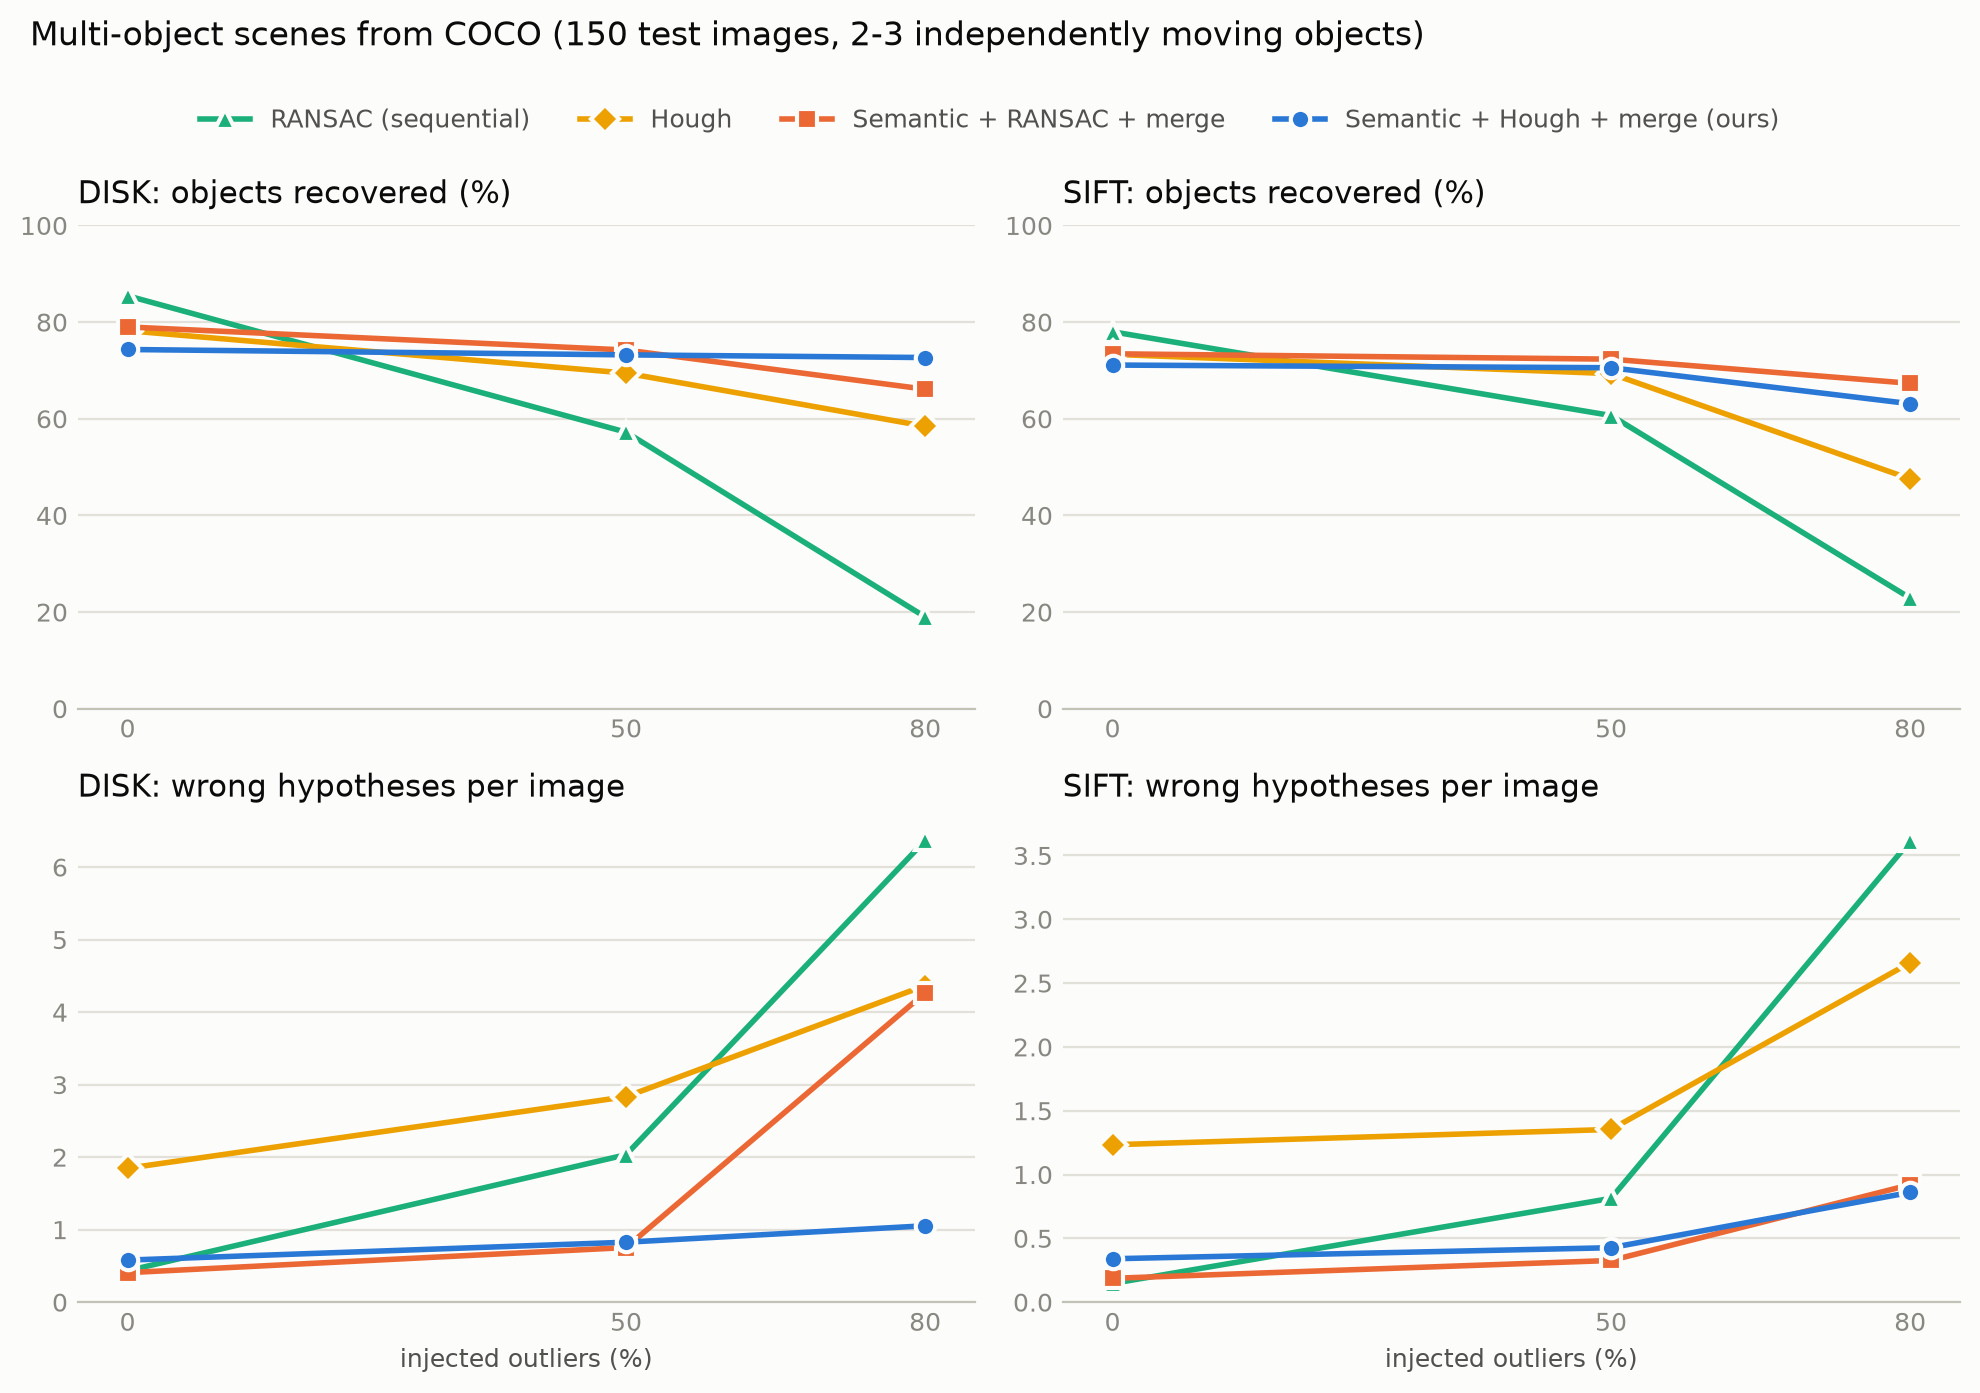
\includegraphics[width=\linewidth]{figures/fig_multiobj.png}
  \caption{Multi-object test split: object recall (top) and wrong hypotheses
  per image (bottom) as outliers are injected.}
  \label{fig:multiobj}
\end{figure}

\paragraph{Results.} Table~\ref{tab:multiobj} and Figure~\ref{fig:multiobj}
show three regimes. \emph{Without injected outliers}, plain sequential RANSAC
is the best method for both features: each object has many matches, which is
the setting RANSAC handles best, and every semantic variant loses some recall
because Mask R-CNN occasionally assigns different classes to the same object
in the two images. \emph{At 50\% outliers}, the semantic methods lead and
Sem+RANSAC+M and Sem+Hough+M are close (DISK: 74.2 vs.\ 73.2 recall, 0.75
vs.\ 0.83 wrong), with Hough about 11$\times$ faster. \emph{At 80\% outliers},
the combination of gating and voting is clearly best with DISK: Sem+Hough+M
recovers 72.7\% of objects with 1.05 wrong hypotheses per image, against
19.0\%/6.37 for RANSAC, 58.4\%/4.37 for Hough alone and 66.1\%/4.27 for
Sem+RANSAC+M, at 17$\times$ lower cost than the latter. With SIFT,
Sem+RANSAC keeps a higher recall at 80\% (67.7 vs.\ 63.1) while the
numbers of wrong hypotheses are similar (0.92 vs.\ 0.86).

The ablation explains the result. Gating alone (Hough $\to$ Sem+Hough) makes
DISK recall almost independent of the outlier rate (74.6, 73.8, 74.2\%)
because injected matches rarely satisfy the same-instance pair rule, but it
leaves duplicates (0.78 per image at 0\%). Merging alone barely changes
ungated methods (Hough $\to$ Hough+M: 1.85 $\to$ 1.57 wrong at 0\%), but
after gating it reduces wrong hypotheses by 1.7--3.9$\times$, because many
``wrong'' hypotheses of gated Hough are partial fits of a motion that another
group already explains. Gating also raises cluster purity, the share of a
hypothesis' inliers that belong to one object, from 92.8\% to 98.1\% on clean
DISK scenes.

\begin{figure}[t]
  \centering
  \begin{subfigure}{0.49\linewidth}
    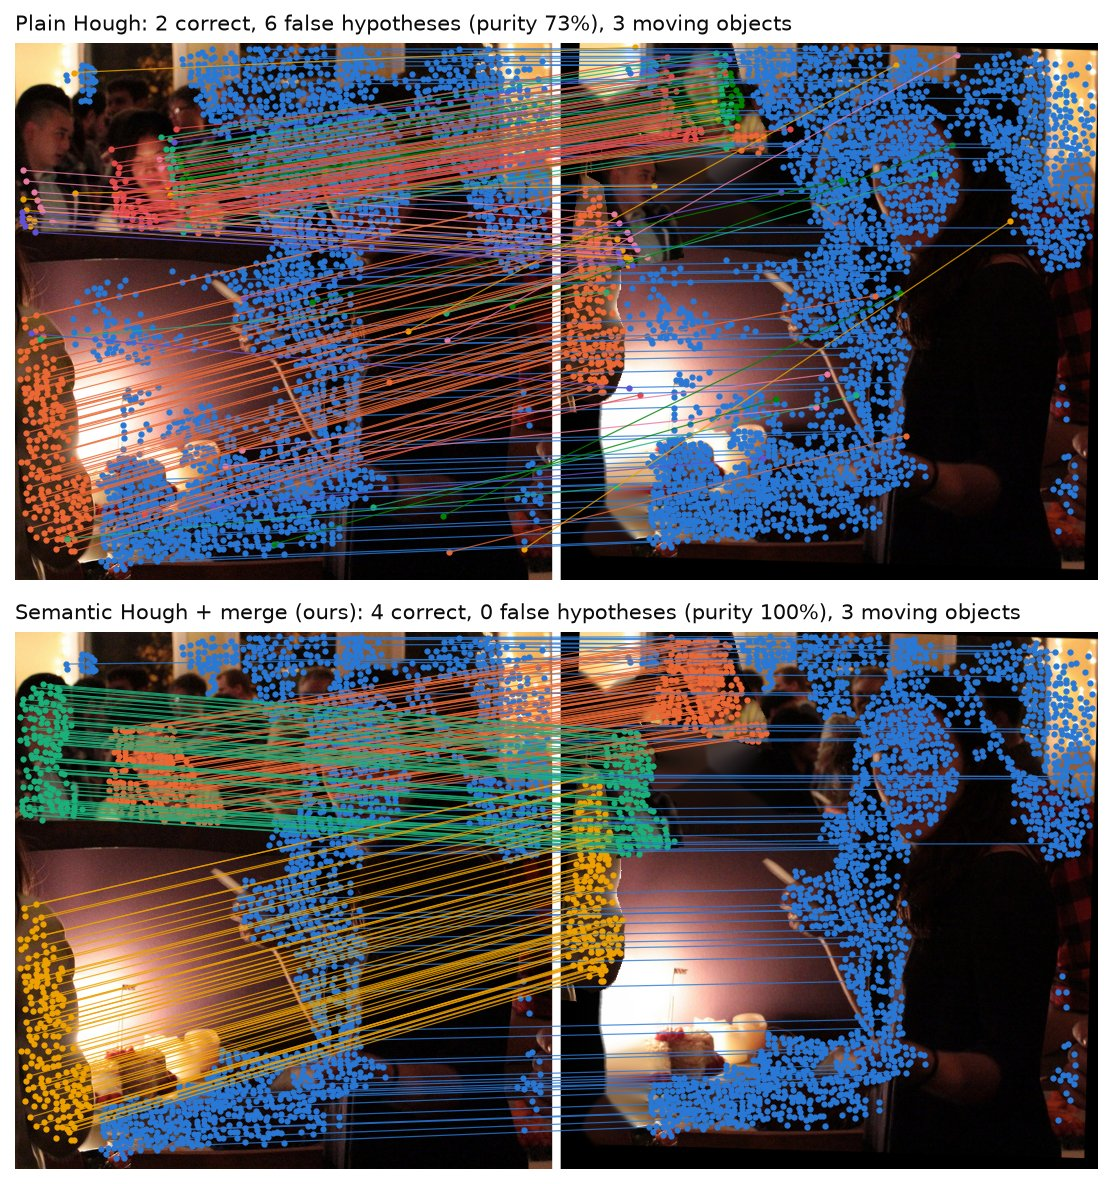
\includegraphics[width=\linewidth]{figures/qual_162092.jpg}
    \caption{Success.}
  \end{subfigure}\hfill
  \begin{subfigure}{0.49\linewidth}
    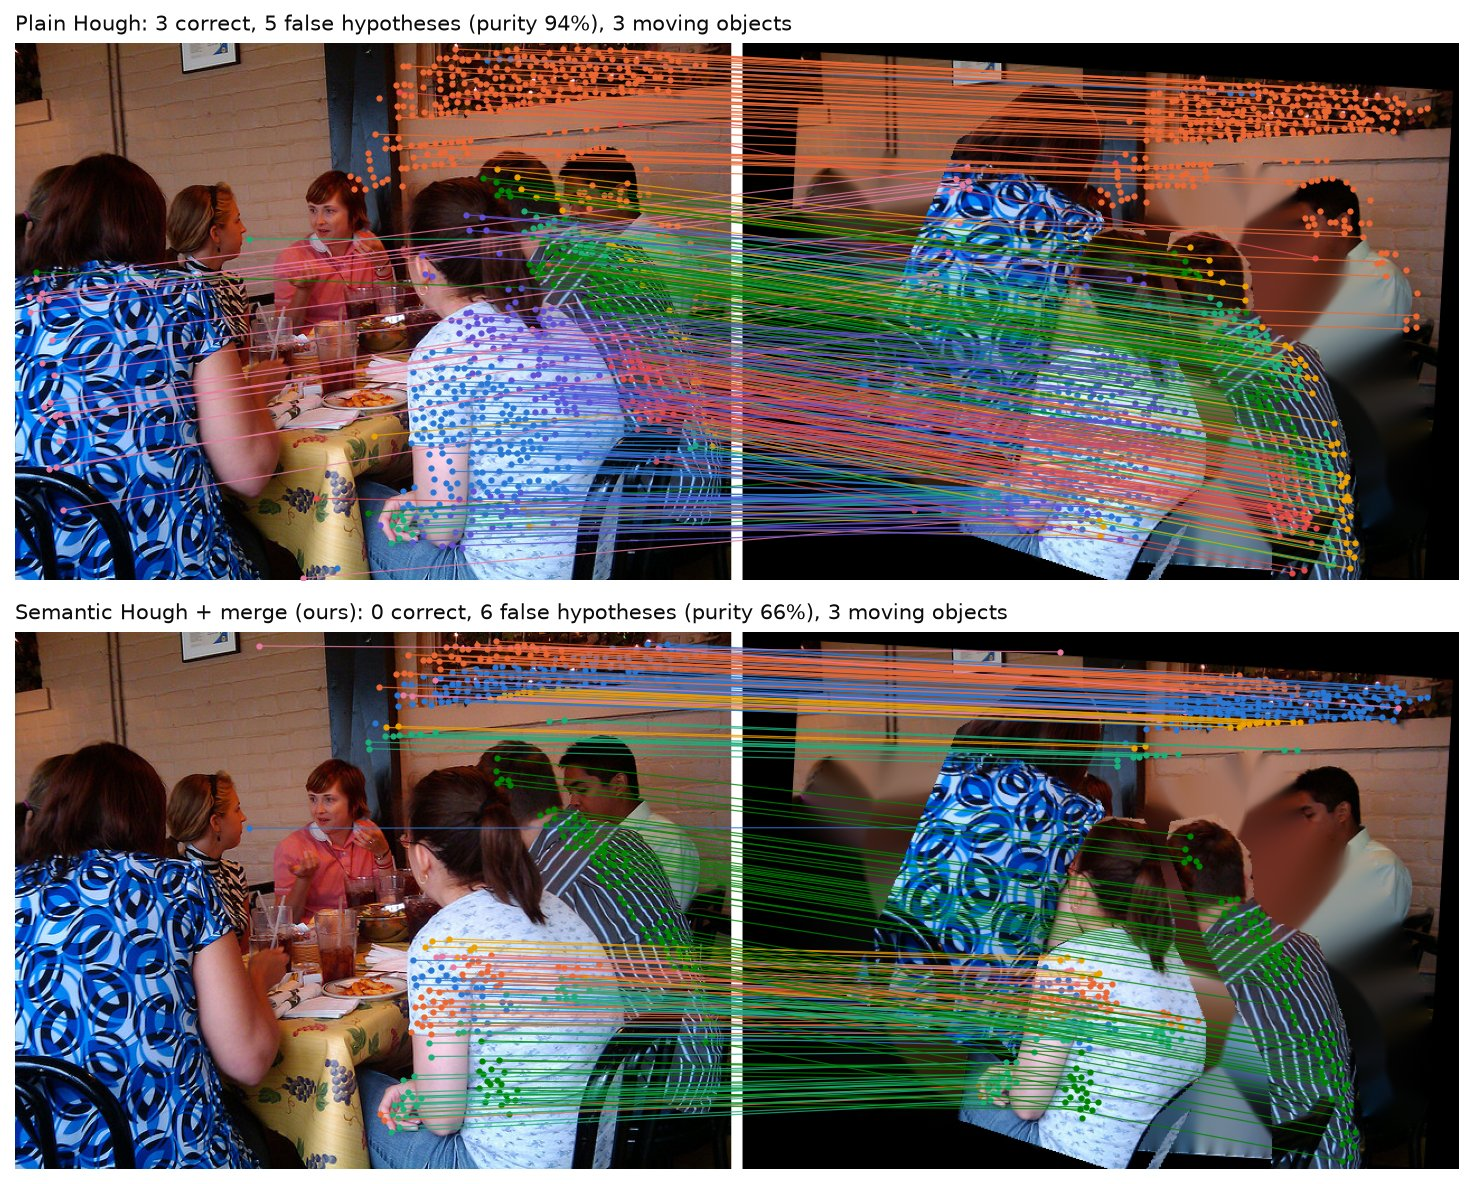
\includegraphics[width=\linewidth]{figures/qual_85157.jpg}
    \caption{Failure.}
  \end{subfigure}
  \caption{Two selected test scenes at 80\% outliers (DISK); top rows plain
  Hough, bottom rows ours. Each colour is one hypothesis. (a) Plain Hough
  returns 6 false hypotheses with 73\% purity; ours recovers all three
  moving objects and the background with none. (b) Three overlapping people
  are moved and one is rotated by about 20$^\circ$; overlapping person
  instances and DISK's lack of rotation invariance make gating group the
  wrong matches, and our method recovers none of the objects.}
  \label{fig:qual}
\end{figure}

\subsection{Variants that did not work}
Several design decisions came from failures, which we report for
completeness.
\begin{itemize}
  \item \textbf{Strict gating.} Treating background as an ordinary class
  rejects every match from a detected object to a region where the detector
  missed it. On the test split (no injected outliers) strict gating reached
  69.6\% DISK recall against 74.6\% for soft gating.
  \item \textbf{Top-60 cluster cap.} An early version visited only the 60
  largest clusters. Gating splits background ``stuff'' into many large
  clusters, which pushed small objects beyond that cap: 69\% of the objects
  lost by gating had a valid cluster ranked below 60. Raising the cap to 300
  for all Hough variants raised gated recall from 60.6\% to 74.6\%.
  \item \textbf{Mask-transfer verification.} We tested rejecting a hypothesis
  when warping its object's mask from $I_1$ with $\mathbf{H}$ does not overlap
  a same-class instance in $I_2$ (IoU $\ge\tau$). On the validation split it
  cost 4--5 points of recall for every method even at $\tau=0.05$, while
  barely reducing wrong hypotheses, because moved objects are often given a
  different class in $I_2$ (R1 alone rejects 9.8\% of correct matches). We
  therefore did not use it.
  \item \textbf{Absolute numbers.} Mask R-CNN detected 95\% of the moved
  objects, so the remaining recall gap between gated and ungated Hough on
  clean scenes is caused by class disagreement between the two images and by
  the rules themselves (14\% of correct pair votes are removed by gating),
  not by missed detections.
\end{itemize}

% =====================================================================
\section{Conclusions}

We made Lowe-style Hough pose clustering work with orientation-free learned
features by voting with pairs of matches, and made pairwise voting robust by
diagnosing and removing the absurd-scale votes created by wrong matches. The
resulting deterministic verifier matches MAGSAC++ on HPatches up to 90\%
outliers and is clearly more accurate at 95\%. For scenes with several
independently moving objects, semantic gating and Hough voting are
complementary: gating removes the cross-object pairs that random outliers
create, and voting tolerates the outliers that remain, so with duplicate
merging the combination keeps DISK object recall between 72.7\% and 74.3\%
from 0\% to 80\% outliers with few wrong hypotheses, where sequential RANSAC falls to
19\%. On clean scenes, however, plain RANSAC remains the most accurate
multi-object method, and on single planes our verifier is slower than the
optimised C++ baselines. The advantage of the approach is therefore
specific to heavily contaminated settings.

\paragraph{Limitations.} DISK, like SuperPoint, is not rotation invariant:
in a synthetic test it fell from 47 matches at 0$^\circ$ in-plane rotation to
10 at 35$^\circ$, while SIFT was unaffected. Our pure-Python Hough
implementation is 40--120$\times$ slower than OpenCV's C++ estimators on
clean data. The outliers are injected synthetically and the multi-object
benchmark is synthetic (pasted objects, planar motions). The semantic prior is
limited to the 80 COCO classes, and overlapping instances of the same class
remain a failure case (Figure~\ref{fig:qual}b).

\paragraph{Future work.}
\begin{enumerate}
  \item \textbf{Identical-instance recognition.} Scenes with many copies of
  one object (retail shelves, bin picking) are a known failure case for
  Hough and RANSAC. Grouping votes by the instance in $I_2$ targets this case
  directly.
  \item \textbf{Open-world gating.} Replacing Mask R-CNN with class-agnostic
  Segment Anything~\cite{kirillov2023sam} masks removes the 80-class limit,
  keeping rules R2 and R3.
  \item \textbf{Learned voting.} A differentiable version of the 16-bin soft
  accumulator would let a network learn per-match vote weights end to end,
  with the present pipeline as its non-learned baseline.
\end{enumerate}

\bibliographystyle{plainnat}
\bibliography{refs}

\end{document}
